\documentclass[11pt]{article}

\usepackage[a4paper,margin=1in]{geometry}
\usepackage[utf8]{inputenc}
\usepackage[T1]{fontenc}
\usepackage{amsfonts}
\usepackage{amsmath}
\usepackage{amssymb}
\usepackage{amsthm}
\usepackage{booktabs}
\usepackage{enumitem}
\usepackage{hyperref}
\usepackage{microtype}
\usepackage{nicefrac}
\usepackage{url}
\usepackage{xcolor}
\definecolor{safebg}{rgb}{0.85,0.93,0.85}
\definecolor{safebd}{rgb}{0.3,0.6,0.3}
\definecolor{unsafebg}{rgb}{0.95,0.85,0.85}
\definecolor{unsafebd}{rgb}{0.7,0.3,0.3}
\definecolor{pendingbg}{rgb}{0.92,0.92,0.95}
\definecolor{pendingbd}{rgb}{0.5,0.5,0.7}
\usepackage{tikz}
\usepackage{pgfplots}
\usetikzlibrary{positioning, arrows.meta, shapes.geometric, fit, calc, matrix}
\pgfplotsset{compat=1.18}
\usepackage[numbers]{natbib}

\newtheorem{definition}{Definition}
\newtheorem{theorem}{Theorem}
\newtheorem{corollary}{Corollary}

\title{Preventing Privilege Escalation in LLM Agents: Provenance-Based Authority in ITES and Conflux}

\author{Raya Buckley}

\date{October 2026}

\begin{document}

\maketitle

\begin{abstract}
Large-language-model agents combine information from multiple principals
while performing externally visible actions. We argue that the system-level
security objective should be privilege escalation, not prompt injection: an
action may proceed only if every principal that influenced it would allow it.
Model-level defences remain probabilistic; this objective is enforced at the
system level and does not rely on model judgement for the confinement decision. We present Influence
Tracking with Extrapolated Security (ITES), which derives each execution's
effective authority from information provenance and the organisation's
existing access-control system, and the System-Level Evaluator for Defences
(SLED), which evaluates declared finite models of a defence under worst-case
model behaviour. Conflux is a reference implementation of ITES with
independent read, authorisation, visibility, and consent decisions,
argument-aware authorisation, audience-specific disclosure, structured
attribution, authenticated dynamic planning, a serialisable verification IR
with cone-of-influence reduction and three depth-unbounded routes over finite
IRs, and a scoped delegation model that remains disabled at runtime. We report
bounded evidence from native SLED mutation testing, semantic agreement across
three encodings of one IR, reduced verification, provenance-rule over-blocking
measurements, and pinned AgentDojo protocol runs reported only as breadth, and
separate it from claims that remain pending. A holding safety verdict is cited
only when the same artefact classifies the invariant as falsifiable under a
declared mutation alphabet. The authority-confinement guarantee---that
authority can only decrease as influence accumulates---follows from the
provenance-based authorisation rule under the stated enforcement and
access-control assumptions, and is independent of language-model behaviour.
\end{abstract}


\section{Introduction}

Large language model (LLM) agents read documents, invoke tools, and perform
externally visible actions on behalf of users. Unlike traditional software,
these agents process natural-language inputs from multiple principals,
including users, documents, databases, APIs, and other systems. Arbitrary
information may influence decisions with real-world consequences
\citep{earlycategorization}.

Prompt injection has emerged as a fundamental challenge
\citep{struq,spotlighting,neuralexec}. Model-level defences improve
instruction following but remain probabilistic: adaptive attacks may
invalidate empirical robustness
\citep{criticaleval,detectprompt,poisoningalignment,checkpointgcg}. We
instead treat \emph{privilege escalation} as the system-level security
objective. Under complete mediation against the current access-control
state, if every principal influencing an action is authorised for it,
arbitrary model behaviour cannot turn that influence into unauthorised
authority \citep{provos2003,davi2010}. The confinement decision is therefore
independent of model judgement; model-level defences remain probabilistic and
are not part of the authority TCB.

We introduce Influence Tracking with Extrapolated Security (ITES), a
provenance-based defence that derives the effective authority of each
execution from information provenance and an existing access-control system,
and the System-Level Evaluator for Defences (SLED), which evaluates
system-level defences under worst-case model behaviour by exhaustively
exploring the declared finite execution space \citep{earlycategorization}. The
historical evaluation explored approximately 1.5 million traces and observed
no successful privilege escalation in the explored finite traces;
Section~\ref{sec:eval} reproduces its per-environment counts exactly under
the recorded depth bound. We do not claim maximal utility: conservative
provenance and independent policy dimensions can deny admissible tasks.

This paper presents ITES and SLED as a system-level framing, and Conflux as a
reference implementation. We do not claim that the individual mechanisms are
new. Capability tracking, argument-level provenance, history-sensitive policy,
and effect-time re-authorisation are prior or concurrent work
\citep{camel,pact,forge,zhu2026runtime,zheng2026apex}; we claim the authority
source and the composition: authority is derived from the organisation's
existing access-control system over the set of influencing principals, and
model judgement is outside the authority TCB for confinement. Our contributions
are:

\begin{enumerate}
  \item We argue that privilege escalation, rather than prompt injection
    itself, is the appropriate system-level security objective for LLM
    agents operating within existing access-control systems.
  \item We present ITES, whose authority-intersection rule is a
    principal-sensitive analogue of low-water-mark integrity
    \citep{biba1977,lomac}, and prove that authority is monotonically
    non-increasing as influence accumulates.
  \item We introduce SLED, which evaluates declared finite models of a defence
    independently of language-model behaviour by exhaustively exploring that
    declared state space under worst-case assumptions.
  \item We describe the Conflux reference architecture, which separates read,
    authorisation, visibility, and consent decisions; implements argument-aware
    policy, audience disclosure, structured attribution, authenticated dynamic
    planning, and serialisable formal verification; and includes a scoped
    delegation model that remains disabled at runtime.
  \item We report evidence at three tiers---reproduced, bounded, and
    pending---covering native SLED mutation testing, semantic agreement across
    three encodings of one IR, cone-of-influence-reduced verification with
    three depth-unbounded routes over finite IRs, provenance-rule over-blocking
    measurement, and pinned AgentDojo protocol runs reported only as breadth.
\end{enumerate}

The remainder of the paper follows that structure.
Section~\ref{sec:threat} states the threat model and the escalation
definition. Section~\ref{sec:ites} gives the authority rule, the
authority-confinement theorem, and its assumptions;
Section~\ref{sec:sled} defines SLED; Section~\ref{sec:conflux} describes
Conflux; Sections~\ref{sec:fv}--\ref{sec:eval} report verification and
evidence.

\section{Related Work}

\subsection{Model-Level Defences}

Model-level defences seek to make language models resist prompt injection
through improved prompting, alignment, or fine-tuning
\citep{struq,spotlighting,secalign,datasentinel}. While often effective
empirically, their security remains probabilistic and may be bypassed by
adaptive attacks \citep{criticaleval,checkpointgcg,poisoningalignment}. ITES
assumes worst-case model behaviour and derives security entirely from
system-level enforcement.

\subsection{System-Level Defences}

Several works address prompt injection through system-level enforcement.
The Dual LLM pattern separates privileged planning from untrusted parsing.
CaMeL extends this with capability tracking and developer-defined policies
enforced by a custom interpreter \citep{camel,designpatterns}. Progent
mediates tool calls with symbolic privilege control \citep{progent}. PACT
tracks argument-level provenance \citep{pact}, and FORGE enforces
history-sensitive Datalog policies \citep{forge}. Effect-time re-authorisation
is also prior art: Zhu and Wang recheck protected effects at an atomic commit
boundary for self-generated subgoals under one principal and one authorisation
root \citep{zhu2026runtime}, and APEX enforces authorised-effect and
task-endorsed-influence conditions at the execution boundary from a contract
compiled before untrusted execution \citep{zheng2026apex}. PACE mediates each
tool call immediately before execution using provenance-aware capabilities and
path confinement \citep{pace}. Agenra provides a policy language with a Lean
enforcement core for stateful agent authorization, tracks value use and
consumed authority, and checks finite-quota policy revisions via simulations
\citep{agenra}. CaMeLoT checks temporal plan properties statically, before
execution \citep{camelot}. PACE and Agenra enforce at runtime; CaMeLoT verifies
plans before execution. All three target system-level properties rather than
model behaviour. ITES differs in the authority source: it derives authority from the organisation's existing
access-control system over the set of influencing principals, rather than from
a single task contract, and keeps model judgement outside the authority TCB.
For authority confinement it does not require a trusted planning model, binary
trust labels, or a new policy language. We claim this authority source and
composition, not the individual mechanisms.

\subsection{Classical Security Lineage}

The ITES authority-intersection rule is structurally analogous to Biba's
low-water-mark contamination: consuming information from an additional
principal can preserve or reduce effective authority but cannot increase it
\citep{biba1977}. LOMAC operationalised low-water-mark integrity in
commodity systems and confronted the same utility--security tension
\citep{lomac}. Denning's lattice model provides the formal foundation: the
intersection of permission sets is a meet in the powerset lattice
\citep{denning1976}. Sabelfeld and Myers provide the vocabulary for
explicit and implicit flows \citep{sabelfeld2003}, while Myers and Liskov's
decentralized information-flow control moves toward multi-principal policies
\citep{myersliskov}. Declassification and endorsement mechanisms
\citep{declassification-survey,robust-declassification,attacker-control,nonmalleable-ifc}
inform Conflux's visibility and disclosure design. Conflux applies this
lineage in an agent setting, with authenticated principal identities and
authority derived from the organisation's current access-control state.

\subsection{Evaluation}

AgentDojo supplies realistic prompt-injection tasks and metrics
\citep{agentdojo}. Existing benchmarks evaluate robustness against known
attacks, while SLED evaluates whether a declared finite model of a defence
satisfies its intended security objective under arbitrary model behaviour.

The next two sections make the privilege-escalation objective precise:
Section~\ref{sec:threat} characterizes the adversary and defines privilege
escalation, and Section~\ref{sec:ites} states the authority rule and the
confinement theorem relative to it.

\begin{table}[h]
\centering
\small
\begin{tabular}{p{2.8cm}p{2.2cm}p{2.2cm}p{2.2cm}p{2.5cm}}
\toprule
& Model-level & Dual LLM & CaMeL & ITES \\
\midrule
Primary mechanism & Model robustness & Model isolation & Dual LLM + policies & Provenance + ACS \\
Security depends on model & Yes & Planning model & Planning model & Confinement: no; judgement: yes \\
Requires new policy language & No & No & Yes & No \\
Tracks & N/A & N/A & Capabilities & Principals \\
Security objective & Prevent PI & Prevent PI & Prevent PI + policies & Prevent PE \\
\bottomrule
\end{tabular}
\caption{Comparison of representative approaches. PI denotes prompt injection; PE denotes privilege escalation; ACS denotes access-control system. For ITES, the final row refers to authority confinement; semantic judgement remains empirical. The table is illustrative, not exhaustive; PACT, FORGE, Zhu and Wang, and APEX occupy nearby points on the authority-source axis.}
\label{tab:comparison}
\end{table}


\section{Threat Model and Security Objective}
\label{sec:threat}

We consider an LLM-based agent that performs externally visible actions on
behalf of users. The agent receives information from multiple principals,
both directly through prompts and indirectly through documents, APIs, and
tool outputs. Any principal may provide arbitrary inputs; we make no
assumptions about the model's ability to distinguish instructions from data
or resist prompt injection. The enforcement mechanism and access-control
system (ACS) are assumed correct and uncompromised.

\subsection{Access-Control System}

We model the ACS as the tuple $(A, U, D, P, W, R)$, where $A$ is the set of
parameterised actions, $U$ is the set of principals, $D$ is the set of data
objects, $P \subseteq U \times A$ is the permission relation, $W
\subseteq D \times U$ specifies authorship, and $R \subseteq D \times U$
specifies read access \citep{abac}. For principal $u$ and action $a$,
$P(u, a)$ holds iff $u$ is authorised to perform $a$.

\subsection{Security Objective}

\begin{definition}[Influencing Principal]
A principal $u$ influences an action if information originating from $u$
contributes, directly or indirectly, to the execution that produces the
action.
\end{definition}

\begin{definition}[Privilege Escalation]
Privilege escalation occurs iff the agent performs an action $a \in A$ for
which there exists an influencing principal $u \in U$ such that $\neg
P(u, a)$.
\end{definition}

Under this formulation, security depends only on provenance and the current
access-control state, not on the source or mechanism of influence. Prompt
injection is one possible source of influence; ITES treats it uniformly with
any other.


\section{ITES: Provenance-Based Authority}
\label{sec:ites}

The central principle of ITES is that every execution inherits the
effective authority implied by the provenance of its inputs. For an
execution $e$ whose direct inputs are data objects $ds \subseteq D$, the
\emph{Principal Context} (influence set in earlier formulations) is:
\[
\mathrm{PC}(e) = \bigcup_{d \in ds} \{u \in U \mid W(d, u)\}.
\]
Objects produced by an execution inherit its complete Principal Context.
Influence accumulates monotonically: once a principal influences a
computation, that influence persists unless a trusted provenance mechanism
removes it. Under the conservative model, influence is never removed.

\subsection{Authorisation Rule}

Given an execution $e$ and an action $a \in A$, let the \emph{decision
context} be the merge of the Principal Context with the provenance of the
action's authority-bearing arguments:
\[
\mathrm{DC}(e,a) = \mathrm{PC}(e) \cup \mathrm{Prov}_{\mathrm{arg}}(a),
\]
where $\mathrm{Prov}_{\mathrm{arg}}(a)$ is the set of principals recorded
for the action's authority-bearing arguments. ITES permits $a$ only if
$\mathrm{DC}(e,a)$ is known and non-empty and
\[
\forall u \in \mathrm{DC}(e,a),\; P(u, a),
\]
and the independent read, visibility, consent, and argument-policy
decisions also allow. Equivalently, the effective authority is the
intersection of the permission sets of all principals in the decision
context. The known-context condition blocks empty and unknown contexts,
preventing vacuous authority.

\subsection{Maximal Authorisation under the Represented Context}

\begin{theorem}[Maximal Authorisation under the Represented Context]
Relative to the represented decision context $\mathrm{DC}(e,a)$ and the
action-authorisation relation $P$, ITES authorises exactly
$\bigcap_{u \in \mathrm{DC}(e,a)} \{a \mid P(u, a)\}$ on that dimension and
no action outside that intersection. Any strict superset under the same $P$
includes an action denied by some principal in $\mathrm{DC}(e,a)$.
\end{theorem}

\begin{proof}[Proof sketch]
By the authorisation rule, ITES authorises exactly the intersection. A
strict superset under the same $P$ must add an action denied by some
principal in $\mathrm{DC}(e,a)$. This is maximality relative to the
represented context and the $P$ dimension. Because $\mathrm{DC}(e,a)$ may
over-approximate the true influencing set, and because read, visibility,
consent, and argument policy are independent dimensions, the theorem does
not assert maximality with respect to all non-escalating actions.
\end{proof}

\subsection{Authority Monotonicity}

\begin{theorem}[Authority Monotonicity]
If $\mathrm{PC}(e_1) \subseteq \mathrm{PC}(e_2)$, then
$\mathrm{Permitted}(\mathrm{PC}(e_2)) \subseteq
\mathrm{Permitted}(\mathrm{PC}(e_1))$.
\end{theorem}

\begin{proof}[Proof sketch]
Adding influencing principals introduces additional constraints; the
intersection can only shrink or remain unchanged.
\end{proof}

\begin{theorem}[System-Level Authority Confinement]
Let $e$ be an execution and let $a$ be an effectful action that $e$
executes. Assume:
\begin{enumerate}
  \item[(A1)] every effectful action is mediated by ITES;
  \item[(A2)] $\mathrm{DC}(e,a)$ contains every principal whose information
        contributed to $e$ or to the authority-bearing arguments of $a$;
  \item[(A3)] for every $u \in \mathrm{DC}(e,a)$, $P(u,a)$ reflects the
        current effective access-control state at execution time;
  \item[(A4)] the executor executes $a$ only with a certificate issued by
        the ITES kernel for a decision over $\mathrm{DC}(e,a)$, bound to
        $a$'s action fingerprint, $\mathrm{DC}(e,a)$'s context fingerprint,
        the executing branch identity, and the current policy versions, and
        revalidated at execution time; and
  \item[(A5)] $\mathrm{DC}(e,a)$ is known and non-empty.
\end{enumerate}
Then $e$ does not perform privilege escalation with respect to $a$, for
arbitrary model behaviour.
\end{theorem}

\begin{proof}[Proof sketch]
By A1 and A4, $a$ is executed only if the ITES kernel accepted it for
$\mathrm{DC}(e,a)$ and the executor revalidated the matching certificate.
By A2, every influencing principal is in $\mathrm{DC}(e,a)$. By A3,
acceptance checked each such principal against the current effective
access-control state. Hence no influencing principal lacks $P(u,a)$, which
is the negation of Definition~2. A5 excludes the empty and unknown cases.
No step depends on the model's proposals.
\end{proof}

The guarantee is independent of the source of influence. Prompt injection,
retrieved documents, untrusted tool outputs, and arbitrary model behaviour
are treated uniformly: once information contributes to an execution, the
authority of that execution is constrained by the permissions of the
corresponding principals. A compromised executor, provenance adapter, or
policy port is not a source of influence; it is a bypass of the trusted
computing base and lies outside A1--A4.

\subsection{Scope of the guarantee}

The theorem is an authority-confinement result, not a claim that every
permitted action is appropriate. ITES bounds the authority available to a
semantic decision but does not decide whether the chosen effect is warranted
by the task or context; that remains empirical. The theorem assumes the
enforcement path, provenance tracking, access-control state, and
authentication are correct. It does not cover a bypass of the mediation
boundary, a provenance error, a stale or incorrect permission, or an
executor that acts without a matching certificate.

It also does not establish policy adequacy: whether the ACS encodes the
organisation's intended restrictions is a separate assurance question. It is
not a non-interference or confidentiality result. Side channels, implicit
flows, and read-based disclosure are outside A1--A5; read, visibility,
consent, and argument policy are independent decisions. Authentication is
part of the trusted computing base: A2 assumes provenance labels correspond
to actual sources. The result is safety-only. Conservative provenance and
independent policy dimensions can deny actions that are consistent with the
ACS, so the theorem does not establish utility or liveness. The relation
$P(u,a)$ is action-level; coarse permission does not imply safe recipients,
amounts, destinations, or argument values. Runtime delegation is disabled,
so $P$ is the explicit ACS; if delegation is activated, $P$ must be the
effective relation $\mathrm{ACS}_{\mathrm{effective}}(e)$. A3 and A4 close
the stale-policy and certificate-binding gaps at recheck, but a race between
recheck and the external effect remains outside the model unless execution
is atomic or fails closed. The finite-IR verification in
Section~\ref{sec:fv} is evidence about the reference IR under declared
bounds, not a proof that the implementation conforms to that IR. These
limits are part of the claim.


\section{SLED: Worst-Case Evaluation}
\label{sec:sled}

Existing prompt-injection benchmarks measure robustness against a finite
collection of attacks. SLED instead evaluates whether a system-level
defence correctly enforces its security properties under arbitrary model
behaviour.

\subsection{State-Space Exploration}

SLED treats each execution as a nondeterministic black box that may produce
any behaviour consistent with the system interface. A system state contains
the environment, the ACS, available data, accumulated influence, pending
executions, and possible actions. Beginning from an initial state, SLED
enumerates every action that may result from each pending execution,
updates the environment, propagates influence, and schedules further
executions. Exploration continues until every reachable state is visited
or a bound is reached.

The Conflux reimplementation provides native SLED with breadth-first
exploration, canonical state keys, deduplication, retained bounds, and
shortest counterexamples. Verdicts are \texttt{SAFE} (exhausted finite
model), \texttt{BOUNDED\_SAFE} (truncated), \texttt{UNSAFE}
(counterexample found), or \texttt{UNKNOWN} (modelling failure). A bounded
verdict is evidence about the retained finite model, not a proof for an
unbounded deployment.


\section{Conflux: Reference Architecture and Extensions}
\label{sec:conflux}

Conflux refactors the original design into a reference security kernel
with one dependency direction and one mediation boundary. Immutable domain
values represent principals, Principal Contexts, permissions, resources,
artefacts, provenance, sessions, and actions. The ITES kernel is pure:
model proposals cannot assert or narrow their Principal Context,
alternative branches share an immutable parent, and effect execution
requires an exact decision certificate.

\subsection{Independent Policy Ports}

Authorisation, read access, visibility, and consent are separate decisions.
Consent cannot override authority; visibility cannot override read policy.
This separation prevents a single policy dimension from manufacturing
authority for another.

\subsection{Argument-Aware Authorisation}

Trusted action-argument roles carry provenance independently of the
proposing execution. Pointwise selector policy checks each principal for
each argument component, preventing authority borrowing through content or
consent.

\subsection{Audience-Specific Disclosure and Attribution}

Deterministic redaction produces audience-specific event views that do not
copy hidden payload fields. Structured attribution records are
evidence-derived rather than model-asserted: trusted model explanations are
rejected in favour of provenance, context, and policy records.

\subsection{Authenticated Dynamic Planning}

Open-ended plans use authenticated operation catalogues, typed bindings,
immutable graph patches, explicit bounded loops, and continuations. Every
grounded effect is re-mediated by ITES at action time; the planner cannot
manufacture authority. Generated code is inert data submitted to a mediated
sandbox capability, not trusted control flow. Security is a hard selection
constraint; eligible plans are then ordered by utility, authority
footprint, sensitive observations, and cost.

\subsection{Scoped Delegation}

The delegation model supports exact issuer, beneficiary, operation,
resource, and argument bindings with expiry, revocation, and atomic
one-use consumption. Delegation remains \emph{runtime-disabled}: ITES still
denies delegation operations. The model exists for bounded verification
only.

\subsection{Serialisable Formal Verification}

A serialisable verification IR supports a reference interpreter, runtime
differential tests, optional Z3 bounded model checking, and a nuXmv
Boolean subset. Property-scoped cone-of-influence (COI) reduction closes
transitively over guards and dependencies. Reduction claims require matching
reference verdicts and a liftable unsafe witness. Section~\ref{sec:fv}
reports the unbounded routes and the falsifiability check that
qualifies every holding verdict.


\section{Formal Verification and Planning}
\label{sec:fv}

SLED-V accepts a finite serialisable transition IR rather than arbitrary
Python. Initial properties cover unauthorised effects and reads, provenance
monotonicity, absence of implicit delegation and bounded resource use.
Bounded SMT results retain solver artefacts; unbounded claims require an
IC3/PDR-capable backend and runtime-to-IR conformance.

Property-scoped cone-of-influence reduction closes transitively over guards
and right-hand-side dependencies that may update an invariant variable.
Reduction claims require matching reference verdicts and a liftable unsafe
witness; an unsupported expression or disagreement fails the comparison. The
retained bundle records matching finite-fixture verdicts and measurable
reduction, while unavailable optional solver binaries contribute no
equivalence evidence.

Authority-constrained planning uses authenticated operation catalogues,
immutable open-ended plan graphs, explicit bounded loops, typed continuations
and value bindings. The evaluation's dynamic-code mode emits an inert
\texttt{ModeledProgram} graph; it is not compiled, evaluated, or sent to an
executor. Every declared effect is re-authorised at modelled action time.
Security is a hard selection constraint; eligible plans are then ordered by
utility, authority footprint, sensitive observations, irreversible effects,
cost and a deterministic fingerprint.

\subsection{Unbounded routes}

Three routes decide an invariant with no step bound on the plan IR.
\texttt{nuxmv-ic3} is IC3/PDR over the finite domain, \texttt{nuxmv-predabs}
is predicate abstraction with CEGAR refinement, and \texttt{nuxmv-msat} is
SMT-based induction. The plan IR declares no step range and keeps the plan's
node bound as a symbolic constant in its guards, so a verdict from any of the
three is not a finite unrolling of a fixed number of steps.

The retained IC3 bundle holds 689 rows: 666 complete and 23 error, with
verdicts \texttt{unsafe} 590, \texttt{safe} 76 and \texttt{unknown} 23. All
23 errors are refusals of models that carry no transition rules; they are
reported as \texttt{unknown}, never as safety. On the plan IR the
predicate-abstraction and induction routes agree with the reference on all
seven rows of the parameter-general bundle (two safe, two unsafe, three
unknown), and each row states its expectation before it is measured. The two
positive rows need an auxiliary invariant plus a transition guard, because
the property alone is not inductive.

A separate bundle reworks the plan-liveness obligation. The earlier
obligation, \texttt{AG(step >= bound -> terminated)}, assigned
\texttt{terminated} inside the abstraction, so a bounded row satisfied it by
construction. The obligation now declares a plan's two good endings and
measures \texttt{step >= bound -> (goal\_reached or safe\_abort)} with the
support invariants \texttt{safe-abort-clean} and \texttt{goal-reached-clean}.
Across 84 measured rows at bounds one to four, every reading meets its stated
expectation, the three routes agree by verdict class on all 28 readings, and
20 of 28 readings carry an unsafe reference verdict, so the agreement cannot
come from a population nothing can refute.

\subsection{Falsifiability of a holding verdict}

A holding verdict (\texttt{safe} or \texttt{bounded\_safe}) is cited as
support only when the same artefact classes the invariant as falsifiable under
a declared mutation alphabet, \texttt{replace\_one\_rule\_guard\_with\_true}.
Each holding invariant receives one class: \texttt{checked}, when a
single-rule guard mutation falsifies it at a reachable state;
\texttt{checked\_by\_construction}, when no such mutation falsifies it; and
\texttt{violated\_at\_baseline} otherwise. Over the defence-model subset, 12
IRs carry 14 invariant rows: four are \texttt{checked}, five
\texttt{checked\_by\_construction} and five \texttt{violated\_at\_baseline}.

The distinction changes what the evaluation may claim. Of the five native
holding rows in the defence bundle only ITES is \texttt{checked} (seven
reachable states, falsified by \texttt{ites-blocks-unauthorised}); Dual-LLM,
CaMeL, PACT and Progent are \texttt{checked\_by\_construction} over two, two,
one and one reachable state, each with a single falsifier whose guard is not
satisfiable at a reachable state. Their holding verdicts are therefore inert
under the declared alphabet and are not cited as support. On the
property-enforcement side six rows are measured and five are refuted; the one
holding row is ITES, and it is \texttt{checked}. The class is a statement
about the declared alphabet, not an absolute property of the invariant.

\begin{figure}[t]
\centering
% Figure 1: property-sensitivity classes
% Generated by scripts/generate_manuscript_figures.py - do not edit by hand.
% input: research/output/runs/defence-models-v1/sensitivity.json sha256=3a6b637f66560bf7b3cf69a753c534998e1fbf5986f5324ec8e5b520e33c9936
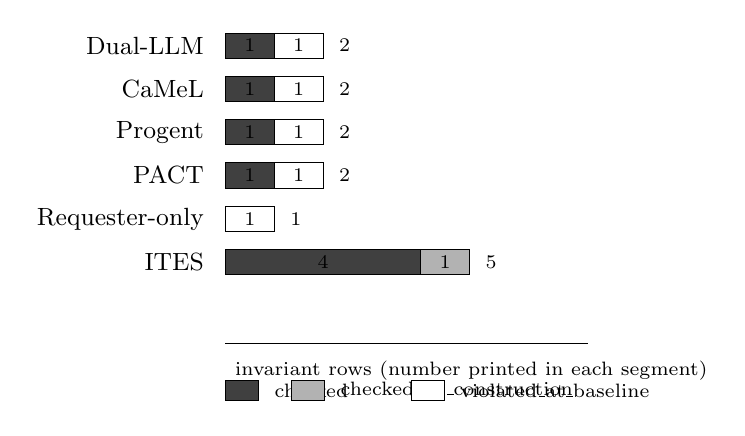
\begin{tikzpicture}[x=1cm,y=1cm]
  \node[anchor=east,font=\small] at (-0.15,0.16) {Dual-LLM};
  \fill[black!75] (0.00,0.00) rectangle +(0.62,0.32);
  \draw[black,line width=0.3pt] (0.00,0.00) rectangle +(0.62,0.32);
  \node[font=\scriptsize] at (0.31,0.16) {1};
  \fill[white] (0.62,0.00) rectangle +(0.62,0.32);
  \draw[black,line width=0.3pt] (0.62,0.00) rectangle +(0.62,0.32);
  \node[font=\scriptsize] at (0.93,0.16) {1};
  \node[anchor=west,font=\scriptsize] at (1.32,0.16) {2};
  \node[anchor=east,font=\small] at (-0.15,-0.39) {CaMeL};
  \fill[black!75] (0.00,-0.55) rectangle +(0.62,0.32);
  \draw[black,line width=0.3pt] (0.00,-0.55) rectangle +(0.62,0.32);
  \node[font=\scriptsize] at (0.31,-0.39) {1};
  \fill[white] (0.62,-0.55) rectangle +(0.62,0.32);
  \draw[black,line width=0.3pt] (0.62,-0.55) rectangle +(0.62,0.32);
  \node[font=\scriptsize] at (0.93,-0.39) {1};
  \node[anchor=west,font=\scriptsize] at (1.32,-0.39) {2};
  \node[anchor=east,font=\small] at (-0.15,-0.94) {Progent};
  \fill[black!75] (0.00,-1.10) rectangle +(0.62,0.32);
  \draw[black,line width=0.3pt] (0.00,-1.10) rectangle +(0.62,0.32);
  \node[font=\scriptsize] at (0.31,-0.94) {1};
  \fill[white] (0.62,-1.10) rectangle +(0.62,0.32);
  \draw[black,line width=0.3pt] (0.62,-1.10) rectangle +(0.62,0.32);
  \node[font=\scriptsize] at (0.93,-0.94) {1};
  \node[anchor=west,font=\scriptsize] at (1.32,-0.94) {2};
  \node[anchor=east,font=\small] at (-0.15,-1.49) {PACT};
  \fill[black!75] (0.00,-1.65) rectangle +(0.62,0.32);
  \draw[black,line width=0.3pt] (0.00,-1.65) rectangle +(0.62,0.32);
  \node[font=\scriptsize] at (0.31,-1.49) {1};
  \fill[white] (0.62,-1.65) rectangle +(0.62,0.32);
  \draw[black,line width=0.3pt] (0.62,-1.65) rectangle +(0.62,0.32);
  \node[font=\scriptsize] at (0.93,-1.49) {1};
  \node[anchor=west,font=\scriptsize] at (1.32,-1.49) {2};
  \node[anchor=east,font=\small] at (-0.15,-2.04) {Requester-only};
  \fill[white] (0.00,-2.20) rectangle +(0.62,0.32);
  \draw[black,line width=0.3pt] (0.00,-2.20) rectangle +(0.62,0.32);
  \node[font=\scriptsize] at (0.31,-2.04) {1};
  \node[anchor=west,font=\scriptsize] at (0.70,-2.04) {1};
  \node[anchor=east,font=\small] at (-0.15,-2.59) {ITES};
  \fill[black!75] (0.00,-2.75) rectangle +(2.48,0.32);
  \draw[black,line width=0.3pt] (0.00,-2.75) rectangle +(2.48,0.32);
  \node[font=\scriptsize] at (1.24,-2.59) {4};
  \fill[black!30] (2.48,-2.75) rectangle +(0.62,0.32);
  \draw[black,line width=0.3pt] (2.48,-2.75) rectangle +(0.62,0.32);
  \node[font=\scriptsize] at (2.79,-2.59) {1};
  \node[anchor=west,font=\scriptsize] at (3.18,-2.59) {5};
  \draw[black,line width=0.4pt] (0,-3.62) -- (4.6,-3.62);
  \node[anchor=north west,font=\scriptsize] at (0,-3.72) {invariant rows (number printed in each segment)};
  \fill[black!75] (0.00,-4.35) rectangle +(0.42,0.26);
  \draw[black,line width=0.3pt] (0.00,-4.35) rectangle +(0.42,0.26);
  \node[anchor=west,font=\scriptsize] at (0.50,-4.22) {checked};
  \fill[black!30] (0.84,-4.35) rectangle +(0.42,0.26);
  \draw[black,line width=0.3pt] (0.84,-4.35) rectangle +(0.42,0.26);
  \node[anchor=west,font=\scriptsize] at (1.34,-4.22) {checked\_by\_construction};
  \fill[white] (2.36,-4.35) rectangle +(0.42,0.26);
  \draw[black,line width=0.3pt] (2.36,-4.35) rectangle +(0.42,0.26);
  \node[anchor=west,font=\scriptsize] at (2.86,-4.22) {violated\_at\_baseline};
\end{tikzpicture}

\caption{Property-sensitivity classes for the six defence models. A segment
counts invariant rows of one class; ITES is the only model whose native
invariants are \texttt{checked}, so it is the only holding verdict in this
subset that may be cited as support. Generated from the retained sensitivity
bundle.}
\label{fig:property-sensitivity}
\end{figure}

\begin{figure}[t]
\centering
% Figure 2: verdict split per unbounded route
% Generated by scripts/generate_manuscript_figures.py - do not edit by hand.
% input: research/output/runs/ic3-unbounded-v1/result.json sha256=433469f9fbb388219e851d64aabbbb0172c129d35b87dcd30bc73a07cf786a2b
% input: research/output/runs/parameter-general-v1/result.json sha256=fdc1d85e3a8eb1015cdf8f496775d03eaf51da99436f0ad390b7233d3bcc109f
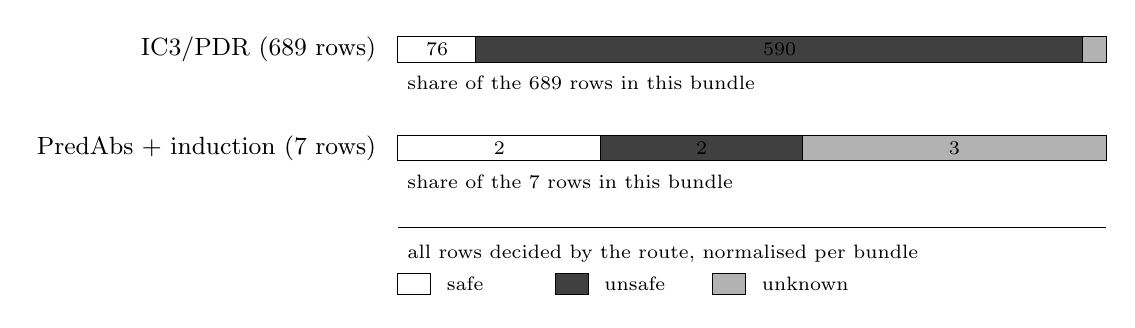
\begin{tikzpicture}[x=1cm,y=1cm]
  \node[anchor=east,font=\small,align=right] at (-0.15,0.16) {IC3/PDR (689 rows)};
  \fill[black!8] (0,0.00) rectangle +(9.0,0.32);
  \fill[white] (0.00,0.00) rectangle +(0.99,0.32);
  \draw[black,line width=0.3pt] (0.00,0.00) rectangle +(0.99,0.32);
  \node[font=\scriptsize] at (0.50,0.16) {76};
  \fill[black!75] (0.99,0.00) rectangle +(7.71,0.32);
  \draw[black,line width=0.3pt] (0.99,0.00) rectangle +(7.71,0.32);
  \node[font=\scriptsize] at (4.85,0.16) {590};
  \fill[black!30] (8.70,0.00) rectangle +(0.30,0.32);
  \draw[black,line width=0.3pt] (8.70,0.00) rectangle +(0.30,0.32);
  \node[anchor=north west,font=\scriptsize] at (0,-0.06) {share of the 689 rows in this bundle};
  \node[anchor=east,font=\small,align=right] at (-0.15,-1.09) {PredAbs + induction (7 rows)};
  \fill[black!8] (0,-1.25) rectangle +(9.0,0.32);
  \fill[white] (0.00,-1.25) rectangle +(2.57,0.32);
  \draw[black,line width=0.3pt] (0.00,-1.25) rectangle +(2.57,0.32);
  \node[font=\scriptsize] at (1.29,-1.09) {2};
  \fill[black!75] (2.57,-1.25) rectangle +(2.57,0.32);
  \draw[black,line width=0.3pt] (2.57,-1.25) rectangle +(2.57,0.32);
  \node[font=\scriptsize] at (3.86,-1.09) {2};
  \fill[black!30] (5.14,-1.25) rectangle +(3.86,0.32);
  \draw[black,line width=0.3pt] (5.14,-1.25) rectangle +(3.86,0.32);
  \node[font=\scriptsize] at (7.07,-1.09) {3};
  \node[anchor=north west,font=\scriptsize] at (0,-1.31) {share of the 7 rows in this bundle};
  \draw[black,line width=0.4pt] (0,-2.1) -- (9.0,-2.1);
  \node[anchor=north west,font=\scriptsize] at (0,-2.2) {all rows decided by the route, normalised per bundle};
  \fill[white] (0.0,-2.95) rectangle +(0.42,0.26);
  \draw[black,line width=0.3pt] (0.0,-2.95) rectangle +(0.42,0.26);
  \node[anchor=west,font=\scriptsize] at (0.50,-2.82) {safe};
  \fill[black!75] (2.0,-2.95) rectangle +(0.42,0.26);
  \draw[black,line width=0.3pt] (2.0,-2.95) rectangle +(0.42,0.26);
  \node[anchor=west,font=\scriptsize] at (2.50,-2.82) {unsafe};
  \fill[black!30] (4.0,-2.95) rectangle +(0.42,0.26);
  \draw[black,line width=0.3pt] (4.0,-2.95) rectangle +(0.42,0.26);
  \node[anchor=west,font=\scriptsize] at (4.50,-2.82) {unknown};
\end{tikzpicture}

\caption{Verdict split per unbounded route, normalised within each bundle so
the two scales can be read together. The IC3/PDR bundle carries 689 rows and
the predicate-abstraction and induction bundle seven; the printed number is
the row count, not a rate. Generated from the two retained result bundles.}
\label{fig:unbounded-routes}
\end{figure}


\section{Evaluation and Evidence Status}
\label{sec:eval}

We distinguish three evidence tiers: \emph{reproduced} (a historical
count re-derived from a retained bundle), \emph{bounded current} (the
reference kernel on finite models), and \emph{pending} (gated on retained
result artefacts). No numerical claim is entered manually; tables and
figures are generated from versioned result JSON, and each generated file
names its source files and their digests in its header.

\subsection{Benchmark Roles and Claim Boundaries}

We use evaluation instruments for three distinct questions and do not pool
them into a single score. Table~\ref{tab:benchmark-boundaries} states what
each can support.

Native SLED is the controlled worst-case instrument. It explores every
behaviour consistent with a declared finite model, so a holding verdict is
evidence about that model and a refutation is a concrete trace. It does not
establish that the implementation conforms to the model, and a finite bound
is not a deployment guarantee.

AgentDojo \citep{agentdojo} is the external comparability instrument. It
contributes realistic indirect-injection protocols, utility accounting, and
targeted attack success. The retained 0.5B, 7B, and 14B runs are pilot and
breadth evidence: no effect tool was executed in any retained bundle, and
the 14B pilot proposed only \texttt{search\_emails}. A full effect-bearing
matrix remains pending and is the pre-submission gate. Until it exists, we
do not use AgentDojo to support a defence or utility-cost claim.

InjecAgent \citep{injecagent} contributes a second injection channel: the
attacker can offer a tool alongside the user's tools, and the benchmark
separates data stealing from direct harm. We retain a no-model
classification of its cases against the authority model. That classification
can say whether a case lies inside or outside the model and whether a policy
decision denies it; it cannot yield a live attack-success or utility number. The 30-case 0.5B run is a plumbing check, not a result.

We do not treat harmfulness-refusal, multi-agent attack-surface, or
task-utility suites as evidence for authority confinement. Their ground truth
is harmful-goal refusal, attack success, or task completion rather than an
authority decision over the set of influencing principals. They may motivate
the problem or test a different property, but they are not substitutes for
the three roles above.

\begin{table}[t]
\centering
\small
\begin{tabular}{@{}p{0.18\linewidth}p{0.27\linewidth}p{0.27\linewidth}p{0.20\linewidth}@{}}
\toprule
Instrument & Question & Retained evidence & Claim boundary \\
\midrule
Native SLED & Does a defence enforce its property for every behaviour in a declared finite model? & Finite-model exploration, mutation kills, and shortest counterexamples & Finite models only; not implementation conformance or deployment safety \\
AgentDojo & Does a defence preserve utility and stop targeted injections in realistic protocols? & Pinned protocol runs at three model scales; all are pilots or breadth evidence & No effect tool executed in retained bundles; full effect-bearing matrix pending \\
InjecAgent & Which principal authorised an effect when an attacker tool is offered? & No-model classification of the benchmark cases against the authority model & Classification only; no live attack-success or utility result \\
\bottomrule
\end{tabular}
\caption{What each evaluation instrument can support. The table is a claim
boundary, not a score: no row is treated as a substitute for another, and
no current AgentDojo pilot is used as defence evidence.}
\label{tab:benchmark-boundaries}
\end{table}

\subsection{Native SLED Reproduction}

The retained native reproduction detects all five seeded monitor defects,
each with a one-step witness, across three fixture pairs with fixed finite
bounds, and reproduces the three historical per-environment trace counts and
their canonical-state compression under the recorded depth bound. The
canonical fixtures are not directly comparable with the archived prototype
(the previous implementation, kept for reference), whose enumeration differed;
Table~\ref{tab:native-sled-reproduction} records both and reports the bound
and the retained count instead of recomputing that prototype's depth-bound
share. This is bounded evidence: it exercises finite
monitor models, not all deployment observers.

% GENERATED FILE -- do not edit by hand.
% Run: python scripts/generate_fourth_year_tables.py
% Source: research/output/runs/native-sled-partb-reproduction-v1/result.json SHA-256: e3751abf62576d85333f08d8f771e56cb11141f195932d1daa5b79fd7d56158c
% Source: research/output/runs/native-sled-reproduction-v1/result.json SHA-256: de42dadd2480a66faf537abd744d117b817f5351c9240d5b368f434df0607657
% Source: research/experiments/baselines/sled-historical-v1.json SHA-256: 66006ebad5998a69a6ba7ba325eef46deb88cc2e1ca2f738259f51010f5de738
\begin{table}[t]
\centering
\small
\begin{tabular}{lrrrlrr}
\toprule
\textbf{Environment} & \textbf{Expected traces} & \textbf{Reproduced} & \textbf{Match} & \textbf{Canonical states} & \textbf{Depth bound} & \textbf{Bound hits} \\
\midrule
env-01 & 422{,}535 & 422{,}535 & yes & 5 & 3 & 0 \\
env-02 & 996{,}451 & 996{,}451 & yes & 17 & 3 & 0 \\
env-03 & 43{,}621 & 43{,}621 & yes & 9 & 3 & 0 \\
\midrule
\textbf{Total} & 1{,}462{,}607 & 1{,}462{,}607 & yes & 31 & 3 & 0 \\
\midrule
\multicolumn{7}{l}{\emph{Canonical fixtures against the archived prototype}} \\
\multicolumn{7}{l}{Pairs compared: 3; negative controls killed: 5 of 5} \\
\multicolumn{7}{l}{Directly comparable with the archived trace claim: no (enumeration\_change)} \\
\multicolumn{7}{l}{Archived depth-bound share: 0.15 (baseline status historical\_unverified)} \\
\multicolumn{7}{l}{The bound-hit count is the retained criterion's structural zero, not a measurement of the archived share} \\
\multicolumn{7}{l}{Runtime is omitted from the deterministic fixture} \\
\bottomrule
\end{tabular}
\caption{Native SLED reproduction. The historical environments reproduce their exact trace counts under the recorded depth bound, and the canonical-state compression collapses the raw traces to a handful of states. The archived prototype enumerated transitions differently, so its headline trace count is not directly comparable; this is reproduction and conformance, not an unbounded security proof. The archived share of traces that reached the bound survives only as an approximate figure from an unverified baseline: the retained runs apply a different criterion and record no trace hitting the bound, so no retained bundle recomputes that share. Counts are read from each bundle's own \texttt{result.json} and the archived share from the recorded baseline.}
\label{tab:native-sled-reproduction}
\end{table}


\subsection{Semantic Conformance}

The reference interpreter and, where the optional binaries are present, the
Z3 and nuXmv backends decide the same bounded IR variants and agree on every
decision, refuted variants included, and the negative control still fails as
designed. Table~\ref{tab:semantic-conformance} counts them. A separate sweep
closes the population instead of listing it: the nine independent delegation
defects have 512 subsets, and the Z3 and nuXmv encodings reproduce the
reference interpreter's verdict class on every one of them, with all three
backends refuting 511. Agreement between the reference interpreter and the
two solver encodings over a closed set of defect combinations is evidence
about the encoding, not a proof of the delegation semantics.

% GENERATED FILE -- do not edit by hand.
% Run: python scripts/generate_fourth_year_tables.py
% Source: research/output/runs/three-way-agreement-v1/result.json SHA-256: 8edf00ec735132107b857d1095e915ccbf76b260233b335f1a87e7ecd8495e2d
\begin{table}[t]
\centering
\small
\begin{tabular}{lr}
\toprule
\textbf{Quantity} & \textbf{Count} \\
\midrule
IR variants checked & 11 \\
Decided by Z3 & 11 \\
Decided by nuXmv & 11 \\
Refuted by the reference interpreter & 10 \\
Reference and Z3 agree & 11 \\
Reference and nuXmv agree & 11 \\
All three agree & 11 \\
Negative control & holds \\
\bottomrule
\end{tabular}
\caption{Semantic conformance over the same bounded IR variants: the reference interpreter, the optional Z3 backend and the optional nuXmv backend decide the same variants and agree on every decision, refuted variants included, and the negative control confirms the harness can still fail. Counts are read from the bundle's own \texttt{result.json}, so the table cannot drift from the evidence it cites.}
\label{tab:semantic-conformance}
\end{table}


\subsection{SLED-V Reduction Scaling}

The retained scaling bundle shows how far the cone-of-influence reduction
shrinks the finite models and that no verdict is downgraded after reduction;
Table~\ref{tab:sledv-scaling} records the sizes and the checks. Two limits
belong with those sizes. The nine fixtures that carry a reference
\emph{unsafe} verdict come from the noise and principal families, not from
the depth family: the five depth fixtures labelled unsafe encode a
single-state model with no transition, and the reference interpreter and Z3
both decide them safe, so the depth family contributes no positive control
and the scaling evidence for it is about reduction size alone. A SLED-V
reduction is bounded evidence on the tested finite models, not a proof for
unbounded deployments.

% GENERATED FILE -- do not edit by hand.
% Run: python scripts/generate_fourth_year_tables.py
% Source: research/output/runs/sledv-scaling-v1/result.json SHA-256: 22f312a535a6ccb7163b1a6f86b6a0f928f1be1366baac5daab54d1d7461d81b
\begin{table}[t]
\centering
\small
\begin{tabular}{lrrrr}
\toprule
\textbf{Family} & \textbf{Fixtures} & \textbf{Largest model} & \textbf{After reduction} & \textbf{Reduction} \\
\midrule
noise scaling & 10 & 41{,}449 & 2 & 20724.5$\times$ \\
principal scaling & 8 & 2{,}517 & 2 & 1258.5$\times$ \\
depth scaling & 10 & 32 & 1 & 32.0$\times$ \\
\midrule
\multicolumn{5}{l}{Total fixtures: 28; COI-equivalent fixtures: 23} \\
\multicolumn{5}{l}{Fixtures the reduction strengthens (bounded safe to safe): 5} \\
\multicolumn{5}{l}{Refuted fixtures: 9; of them in the depth family: 0} \\
\multicolumn{5}{l}{Verdict downgrades after reduction: none} \\
\multicolumn{5}{l}{Reference and Z3 agree: yes} \\
\bottomrule
\end{tabular}
\caption{SLED-V reduction over three scaling families. The reduction collapses the finite models by up to the factor shown, no verdict is downgraded after reduction, and the reference and Z3 decisions agree. Sizes and checks are read from the bundle's own \texttt{result.json}. The reduction strengthens five fixtures from bounded safe to safe, and every refuted fixture comes from the noise or principal family: the five depth fixtures labelled unsafe encode a single state and no transition, so they give the reduction no positive control and the depth family's evidence is about reduction size alone. This is bounded evidence on the tested finite models; it is not a proof of security for arbitrary or unbounded deployments.}
\label{tab:sledv-scaling}
\end{table}


\subsection{Over-blocking and Capability Retention}

The retained provenance bundle compares three provenance rules over 351
symbolic delegation fixtures. The conservative rule denies 35 of the 208
securely achievable fixtures, and the authenticated rule denies none of them,
while the mean size of the computed provenance set falls from 8.62 to 3.08;
the requester-only control shows what the confinement rule costs rather than
a capability figure. Table~\ref{tab:provenance-precision} records the counts.
The measurement is one-sided: the bundle counts the denials the rule
produces, holds no refusal counter and no model, so a refusal an agent would
add on top is uncounted. The denials concentrate where provenance
heterogeneity is high: 24 of 32 fixtures there, against none of 117 at low
heterogeneity.

% GENERATED FILE -- do not edit by hand.
% Run: python scripts/generate_fourth_year_tables.py
% Source: research/output/runs/provenance-precision-v1/result.json SHA-256: 63e1c91896aa9090c95aff93dfe1fad102157d032bb4fba739f7d19bcdea4082
\begin{table}[t]
\centering
\small
\begin{tabular}{llrrrr}
\toprule
\textbf{Provenance rule} & \textbf{Provenance set} & \textbf{Mean size} & \textbf{Secure tasks completed} & \textbf{False denials} & \textbf{Vulnerable executions} \\
\midrule
C0 requester only (negative control) & requester & 1.00 & 208 of 208 & 0 of 208 & 48 of 48 \\
C1 may-have-written provenance & possible authors & 8.62 & 173 of 208 & 35 of 208 & 0 of 48 \\
C2 authenticated provenance & actual contributors & 3.08 & 208 of 208 & 0 of 208 & 0 of 48 \\
\bottomrule
\end{tabular}
\caption{Capability retention and over-blocking for three provenance rules over 351 symbolic delegation fixtures (208 securely achievable, 95 securely blocked, 48 vulnerable), three repetitions per parameter cell. C0 is the negative control: it authorises the requester alone, so its row shows what the confinement rule costs rather than a capability figure. From the conservative rule to authenticated provenance, denials of securely achievable work fall from 35 to 0, the mean size of the computed provenance set falls from 8.62 to 3.08, and 0 of 351 authenticated rows both authorise and violate the confinement rule. The measurement is one-sided: the rows count the denials the rule produces, and the bundle holds no refusal counter and no model, so a refusal an agent would add on top is uncounted.}
\label{tab:provenance-precision}
\end{table}


\subsection{Direction Security Models}

The retained, checksummed bundle reports safe exhaustion for the canonical
finite disclosure and delegation models and minimal witnesses for every
seeded selector, disclosure, attribution, and delegation defect. Delegation
remains disabled at runtime, so these are bounded-model statements about the
models, not operational findings.

\subsection{Real Models and AgentDojo}

The pinned AgentDojo adapter (package \texttt{0.1.35}, benchmark
\texttt{v1.2.2}) provides the retained breadth evidence counted in
Table~\ref{tab:agentdojo-breadth}, with the protocol identity of each bundle
in Table~\ref{tab:agentdojo-fingerprints}. Both tables are generated from the
retained result and protocol JSON. They record what a 0.5B floor model did,
not a defence result: at this model scale utility is zero, so the security
counts carry no signal, and the standing limitation is stated in the table
caption. The two 7B runs in the same ledger share a second, independent
limit: their five tasks are read-only, their ground truth is
\texttt{search\_emails} alone, and every retained log made at most that one
call, so no effect tool was reached at any model size and their security
counts carry no signal either. Of the 97 user tasks in the four suites, 60
require an effect call. That 60-task subset is a selection frame, not a
result: no effect call has
been executed in any retained AgentDojo cell. The retained pilots use one
repetition and one seed, and a single pass cannot support a utility-cost
estimate. Real-model and AgentDojo claims stay bounded until a capable model
completes the protocols on effect-bearing tasks.

% GENERATED FILE -- do not edit by hand.
% Run: python scripts/generate_fourth_year_tables.py
% Source: research/output/runs/agentdojo-stratified-banking-v1/result.json SHA-256: 17edd75b1b5e6e03df835154457b60de3dff6c4f963020c7dd38c3bdd57777fa
% Source: research/output/runs/agentdojo-stratified-banking-v1/protocol.json SHA-256: cbf41d0ae0242311fadf67b2340a723cd06c20a26a3d11b1ec25ca5ade1e8cf1
% Source: research/output/runs/agentdojo-stratified-slack-v1/result.json SHA-256: 69e60b580d24bf9a28796d267e5434ec5afb9d664fe7dd697019fa47ccff2b15
% Source: research/output/runs/agentdojo-stratified-slack-v1/protocol.json SHA-256: 9c2ce6e181a17faaf96f061039b3cce5c9c209d965d17cd4951f7819a405946d
% Source: research/output/runs/agentdojo-stratified-travel-v1/result.json SHA-256: a4e85c02b7533a8ff71f536aca87b5a4594ad6467ff4828f5a99c004fc91a6d1
% Source: research/output/runs/agentdojo-stratified-travel-v1/protocol.json SHA-256: ee62fbc6ae0fbf0f4dcf6dcddc8e9e57a95db3693b67e8ec37c9498c5135fa5c
% Source: research/output/runs/agentdojo-stratified-workspace-v1/result.json SHA-256: 810e24057e8b961f49ae88c1b47901049b2443a5116c2057a0c099adcafb70ce
% Source: research/output/runs/agentdojo-stratified-workspace-v1/protocol.json SHA-256: 1d75d38896dc76d9d0a8071143f67fe0d05ade74acb620a4a8fd2cd80f6a711b
% Source: research/output/runs/agentdojo-pilot-banking-v1/result.json SHA-256: 7e74dfa894f89d13e1db9e35495b484c6e47eae4ad8bc4195608a79633983ab0
% Source: research/output/runs/agentdojo-pilot-banking-v1/protocol.json SHA-256: 44904393e0c13f582f1116bc1ed4c3c0227da55c87252ce50d5e7d709b0830a1
\begin{table}[t]
\centering
\small
\begin{tabular}{llrrrrl}
\toprule
\textbf{Run} & \textbf{Cells} & \textbf{Complete} & \textbf{Utility} & \textbf{Security} & \textbf{Incomplete} & \textbf{Failure categories} \\
\midrule
banking (\textit{stratified}, 4 tasks) & 24 & 24 & 0 & 24 & 0 & utility 24 \\
slack (\textit{stratified}, 5 tasks) & 30 & 24 & 0 & 24 & 6 & model 6, policy 6, utility 24 \\
travel (\textit{stratified}, 10 tasks) & 60 & 60 & 0 & 60 & 0 & policy 42, utility 60 \\
workspace (\textit{stratified}, 13 tasks) & 78 & 78 & 0 & 78 & 0 & policy 8, utility 78 \\
banking (\textit{pilot}, 2 tasks) & 12 & 12 & 0 & 12 & 0 & utility 12 \\
\textbf{Total} & \textbf{204} & \textbf{198} & \textbf{0} & \textbf{198} & \textbf{6} & \\
\bottomrule
\end{tabular}
\caption{Retained AgentDojo breadth evidence, counted from each bundle's own \texttt{result.json}. 204 cells, 198 complete, 0 with utility, 198 reporting no security violation. The model is a 0.5B floor configuration, so utility is zero and the security counts are vacuous: a model that completes no task cannot be shown to be protected. Failure counts are the categories the run recorded: each cell contributes one count per recorded failure, so one cell can carry several categories and a cell that completed can still carry a category such as \texttt{utility}. The six incomplete slack cells were later diagnosed as capability failures of that model, not adapter gaps; a module rerun of the same suite reports them as parser failures.}
\label{tab:agentdojo-breadth}
\end{table}


% GENERATED FILE -- do not edit by hand.
% Run: python scripts/generate_fourth_year_tables.py
% Source: research/output/runs/agentdojo-stratified-banking-v1/result.json SHA-256: 17edd75b1b5e6e03df835154457b60de3dff6c4f963020c7dd38c3bdd57777fa
% Source: research/output/runs/agentdojo-stratified-banking-v1/protocol.json SHA-256: cbf41d0ae0242311fadf67b2340a723cd06c20a26a3d11b1ec25ca5ade1e8cf1
% Source: research/output/runs/agentdojo-stratified-slack-v1/result.json SHA-256: 69e60b580d24bf9a28796d267e5434ec5afb9d664fe7dd697019fa47ccff2b15
% Source: research/output/runs/agentdojo-stratified-slack-v1/protocol.json SHA-256: 9c2ce6e181a17faaf96f061039b3cce5c9c209d965d17cd4951f7819a405946d
% Source: research/output/runs/agentdojo-stratified-travel-v1/result.json SHA-256: a4e85c02b7533a8ff71f536aca87b5a4594ad6467ff4828f5a99c004fc91a6d1
% Source: research/output/runs/agentdojo-stratified-travel-v1/protocol.json SHA-256: ee62fbc6ae0fbf0f4dcf6dcddc8e9e57a95db3693b67e8ec37c9498c5135fa5c
% Source: research/output/runs/agentdojo-stratified-workspace-v1/result.json SHA-256: 810e24057e8b961f49ae88c1b47901049b2443a5116c2057a0c099adcafb70ce
% Source: research/output/runs/agentdojo-stratified-workspace-v1/protocol.json SHA-256: 1d75d38896dc76d9d0a8071143f67fe0d05ade74acb620a4a8fd2cd80f6a711b
% Source: research/output/runs/agentdojo-pilot-banking-v1/result.json SHA-256: 7e74dfa894f89d13e1db9e35495b484c6e47eae4ad8bc4195608a79633983ab0
% Source: research/output/runs/agentdojo-pilot-banking-v1/protocol.json SHA-256: 44904393e0c13f582f1116bc1ed4c3c0227da55c87252ce50d5e7d709b0830a1
\begin{table}[t]
\centering
\small
\begin{tabular}{lllll}
\toprule
\textbf{Bundle} & \textbf{Protocol suite id} & \textbf{Source commit} & \textbf{Fingerprint} & \textbf{Model} \\
\midrule
agentdojo-stratified-banking-v1 & banking:expanded:user\_task\_0 & \texttt{1127281372dc} & \texttt{da3024092bc533e8} & Qwen/Qwen2.5-0.5B-Instruct \\
agentdojo-stratified-slack-v1 & slack:expanded:user\_task\_0 & \texttt{1127281372dc} & \texttt{936563e1782d1001} & Qwen/Qwen2.5-0.5B-Instruct \\
agentdojo-stratified-travel-v1 & travel:expanded:user\_task\_0 & \texttt{1127281372dc} & \texttt{54781fe7e475522b} & Qwen/Qwen2.5-0.5B-Instruct \\
agentdojo-stratified-workspace-v1 & workspace:expanded:user\_task\_0 & \texttt{1127281372dc} & \texttt{cbe8f9ad9a5f1b8b} & Qwen/Qwen2.5-0.5B-Instruct \\
agentdojo-pilot-banking-v1 & banking:expanded:user\_task\_0 & \texttt{1127281372dc} & \texttt{185539f9d2650759} & Qwen/Qwen2.5-0.5B-Instruct \\
\bottomrule
\end{tabular}
\caption{Protocol identity of the retained bundles. A repeat that changes the suite, task set, bounds, model identity, prompts, or inputs changes the fingerprint, so a matching fingerprint is what makes a rerun comparable; a matching fingerprint also implies the recorded source commit. The fingerprints are truncated to their first 16 hexadecimal digits here and kept whole in each bundle's \texttt{result.json}. The stratified bundles were retained before the sweep passed the selection's own suite id, so their suite ids use the earlier \texttt{<suite>:expanded:<first task>} spelling rather than the selection manifest's \texttt{<suite>:stratified-v1}; every id here is the one the run recorded.}
\label{tab:agentdojo-fingerprints}
\end{table}


\subsection{Remote AgentDojo runs on a local 14B model}

The pinned adapter was also run with a single local model,
\texttt{Qwen/Qwen2.5-14B-Instruct} (revision \texttt{cf98f3b3}), served in
4-bit NF4 on one CUDA device at temperature $0.0$ and seed $0$. Three runs
were retained: a workspace pilot of 30 cells, and a stratified sweep of 24
banking cells and 78 workspace cells. Every cell ran; all but one completed,
and the single incomplete cell is a parser failure.

In the pilot, native utility is $18/30$ and identical across the three arms
(\texttt{no\_defence}, \texttt{ites\_conservative}, \texttt{ites\_oracle},
$6/10$ each): the guarded arms neither gain nor lose a completed user task.
The recorded failures are \texttt{utility}~(12) and \texttt{policy}~(3), with
no model, parser, tool, setup, security or bound failure. The three policy
failures are all \texttt{user\_task\_39} under the two guarded arms, where the
arm refused a repeated \texttt{search\_emails} call.

The security counts must be read with their floor in view. Over the whole
pilot the model proposed one tool only, \texttt{search\_emails}, 65 times, and
the 30 executed mediation records are all that read tool. No effect call --- a
write, send or delete --- was proposed in any cell, so none was executed. The
counts therefore describe this model and this harness, not a defence that
stopped an attempted injection.

The two stratified runs are weaker and are reported as such. The banking
sweep recorded zero utility and 192 mediation records that are all refused
with the adapter-level reason \texttt{unsupported\_tool}, so every call is
refused before the policy engine is consulted and the per-arm ``secure'' rate
is vacuous. The workspace sweep recorded utility $1/78$ and 564 records: 348
\texttt{provider\_failed}, 177 blocked and 39 executed, all of them
\texttt{search\_emails}; in 54 of the 78 cells nothing executed. Resident
failure categories are \texttt{utility}~(76), \texttt{policy}~(46) and
\texttt{parser}~(1).

\begin{figure}[t]
\centering
% Figure 3: runpod cells per arm and per stratum
% Generated by scripts/generate_manuscript_figures.py - do not edit by hand.
% input: research/output/runs/runpod-h100-14b-v1/result.json sha256=75088503543ad7b678f6922d2d5d0aacd34bc531fabc88124a1b1900cce8048e
% input: research/output/runs/runpod-h100-14b-stratified/agentdojo-stratified-banking-v1/result.json sha256=094eede6e6dcabe36af7cde9c9e324838490e2e767799c6cd0ca4efccc0df4e6
% input: research/output/runs/runpod-h100-14b-stratified/agentdojo-stratified-workspace-v1/result.json sha256=927a64eaf68fe45cb8a23957bdce0e944bfdff372fe0e054ff49429867ad0180
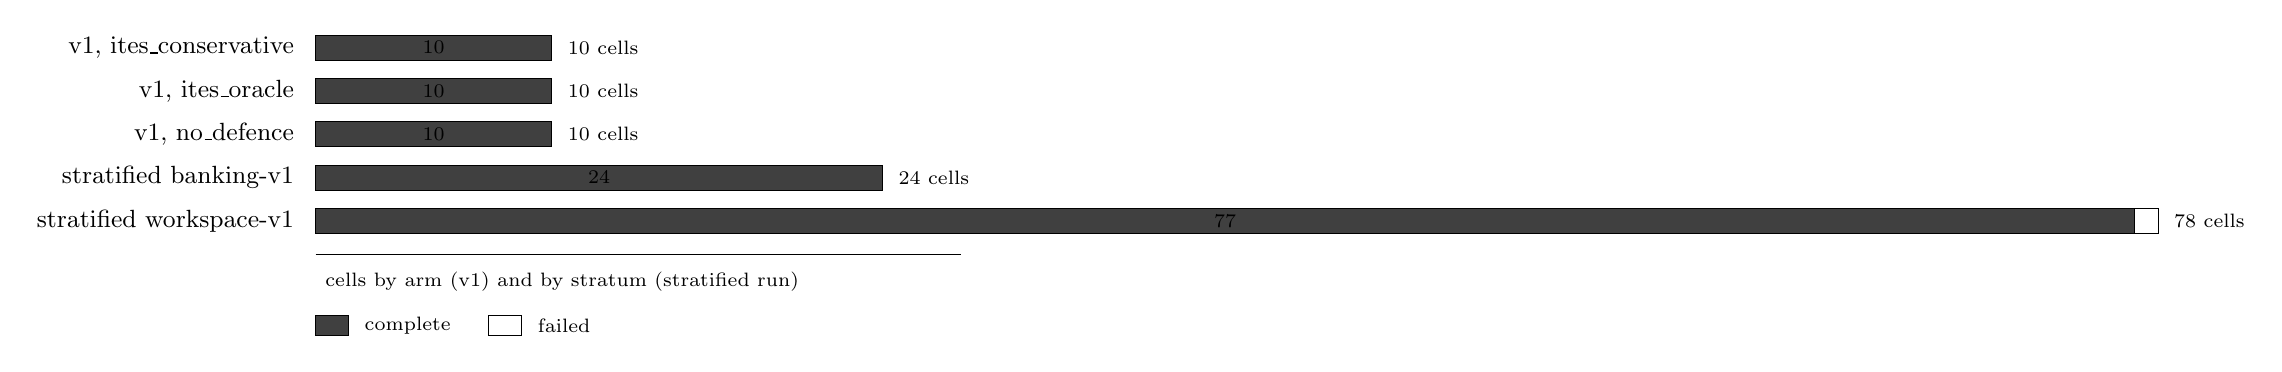
\begin{tikzpicture}[x=1cm,y=1cm]
  \node[anchor=east,font=\small] at (-0.15,0.16) {v1, ites\_conservative};
  \fill[black!75] (0.00,0.00) rectangle +(3.00,0.32);
  \draw[black,line width=0.3pt] (0.00,0.00) rectangle +(3.00,0.32);
  \node[font=\scriptsize] at (1.50,0.16) {10};
  \node[anchor=west,font=\scriptsize] at (3.08,0.16) {10 cells};
  \node[anchor=east,font=\small] at (-0.15,-0.39) {v1, ites\_oracle};
  \fill[black!75] (0.00,-0.55) rectangle +(3.00,0.32);
  \draw[black,line width=0.3pt] (0.00,-0.55) rectangle +(3.00,0.32);
  \node[font=\scriptsize] at (1.50,-0.39) {10};
  \node[anchor=west,font=\scriptsize] at (3.08,-0.39) {10 cells};
  \node[anchor=east,font=\small] at (-0.15,-0.94) {v1, no\_defence};
  \fill[black!75] (0.00,-1.10) rectangle +(3.00,0.32);
  \draw[black,line width=0.3pt] (0.00,-1.10) rectangle +(3.00,0.32);
  \node[font=\scriptsize] at (1.50,-0.94) {10};
  \node[anchor=west,font=\scriptsize] at (3.08,-0.94) {10 cells};
  \node[anchor=east,font=\small] at (-0.15,-1.49) {stratified banking-v1};
  \fill[black!75] (0.00,-1.65) rectangle +(7.20,0.32);
  \draw[black,line width=0.3pt] (0.00,-1.65) rectangle +(7.20,0.32);
  \node[font=\scriptsize] at (3.60,-1.49) {24};
  \node[anchor=west,font=\scriptsize] at (7.28,-1.49) {24 cells};
  \node[anchor=east,font=\small] at (-0.15,-2.04) {stratified workspace-v1};
  \fill[black!75] (0.00,-2.20) rectangle +(23.10,0.32);
  \draw[black,line width=0.3pt] (0.00,-2.20) rectangle +(23.10,0.32);
  \node[font=\scriptsize] at (11.55,-2.04) {77};
  \fill[white] (23.10,-2.20) rectangle +(0.30,0.32);
  \draw[black,line width=0.3pt] (23.10,-2.20) rectangle +(0.30,0.32);
  \node[anchor=west,font=\scriptsize] at (23.48,-2.04) {78 cells};
  \draw[black,line width=0.4pt] (0,-2.47) -- (8.2,-2.47);
  \node[anchor=north west,font=\scriptsize] at (0,-2.57) {cells by arm (v1) and by stratum (stratified run)};
  \fill[black!75] (0.0,-3.50) rectangle +(0.42,0.26);
  \draw[black,line width=0.3pt] (0.0,-3.50) rectangle +(0.42,0.26);
  \node[anchor=west,font=\scriptsize] at (0.50,-3.37) {complete};
  \fill[white] (2.2,-3.50) rectangle +(0.42,0.26);
  \draw[black,line width=0.3pt] (2.2,-3.50) rectangle +(0.42,0.26);
  \node[anchor=west,font=\scriptsize] at (2.70,-3.37) {failed};
\end{tikzpicture}

\caption{Cells by arm for the 14B pilot and by stratum for the stratified
sweep. A segment counts cells; the grey segment is completed cells and the
outlined segment failed cells. The banking stratum completed every cell while
executing nothing, which is why its security count carries no efficacy claim.
Generated from the three retained run bundles.}
\label{fig:runpod-cells}
\end{figure}

\subsection{Refusal attribution}

The retained bundles name the rule behind each refusal without a rerun. One
bundle re-derives the causing rule from the report that every blocked record
already keeps, and attributes 93 refused calls in the six bundles that hold
them: \texttt{snapshot-read-policy} 60 on the read dimension,
\texttt{in-memory-authorisation} 29 and \texttt{in-memory-argument-policy} 4
on the authorisation dimension, over the tools \texttt{search\_emails} 81 and
\texttt{delete\_file} 12, with the conservative arm holding 57 of the 93. A
refusal count is therefore legible as a named rule, so the snapshot-read,
authorisation and argument-policy layers can be told apart in retained
evidence.


\section{Discussion and Limitations}

Conflux assumes sound authentication, provenance, policy state, and complete
mediation. It does not prevent actions authorised for every influencing
principal and does not guarantee subjective intent alignment. Conservative
contexts can over-approximate influence, reducing utility. The
authority-intersection rule is a meet in the powerset lattice and is
structurally analogous to Biba's low-water-mark contamination
\citep{biba1977,denning1976}. It is not a new lattice construction. Our claim
is the system-level objective and the composition with an existing
access-control system; the information-flow lineage
\citep{sabelfeld2003,myersliskov,declassification-survey,robust-declassification,attacker-control,nonmalleable-ifc}
supplies the vocabulary and the limits.

We do not claim a new access-control model, a new policy language, or a
model-level defence. We do not claim that effect-time re-authorisation is new;
concurrent work enforces authorised effects at execution boundaries
\citep{zhu2026runtime,zheng2026apex}. We do not claim a proof about the
implementation or an unbounded deployment: the formal results are scoped to
declared finite IRs, the stated assumptions, and the retained conformance
evidence. The claim is the authority source, the architecture, and the scoped
evidence.

Authorised-read safety is not noninterference: a system can obey local ACL
checks and still leak information through outputs or control flow. Formal
results are scoped to their finite model, backend, and conformance
evidence: a holding verdict is cited only when the same artefact classifies
the invariant as falsifiable under a declared mutation alphabet, so an
inert holding row is not offered as support. Delegation has a bounded model
and lifecycle representation but remains unsupported by operational ITES.
Provider adapters are research prototypes, not production isolation
boundaries. Effect-bearing real-model and AgentDojo comparisons remain pending
until gated runs produce retained evidence. The retained AgentDojo runs are
breadth evidence, read with their capability floor in view rather than as a
defence result. Planning comparisons also remain pending.


\section{Conclusion}

The paper makes four connected claims and reports one evidence contribution.
First, privilege escalation, not prompt injection alone, is the right
system-level objective for LLM agents. Second, ITES meets that objective by
deriving authority from information provenance and the organisation's existing
access-control system; authority can only decrease as influence accumulates,
given correct enforcement, provenance coverage, and current access-control
state, independently of language-model behaviour. Third, SLED evaluates
declared finite models of a defence under worst-case model behaviour, so a
falsifiable holding verdict is evidence about that model rather than about
deployment. Fourth, Conflux is a reference
implementation that separates read, authorisation, visibility, and consent,
and extends the design to argument-aware policy, disclosure, attribution,
planning, and finite-IR verification. The fifth contribution is the evidence
report: reproduced and bounded results across native SLED mutation testing,
semantic agreement, reduced verification, provenance-rule over-blocking, and
pinned AgentDojo breadth runs, with remaining claims explicitly pending. We do not claim broad
novelty: capability tracking, argument-level provenance, history-sensitive
policy, and effect-time re-authorisation are prior or concurrent work. The evidence is scoped to declared finite models and retained
bundles; real-model and external-benchmark results remain breadth or pending,
and delegation remains disabled at runtime. The next step is stronger
evidence, not a stronger claim.


\bibliography{references}
\bibliographystyle{plainnat}

\end{document}
